% Created by tikzDevice version 0.12 on 2019-02-08 11:09:19
% !TEX encoding = UTF-8 Unicode
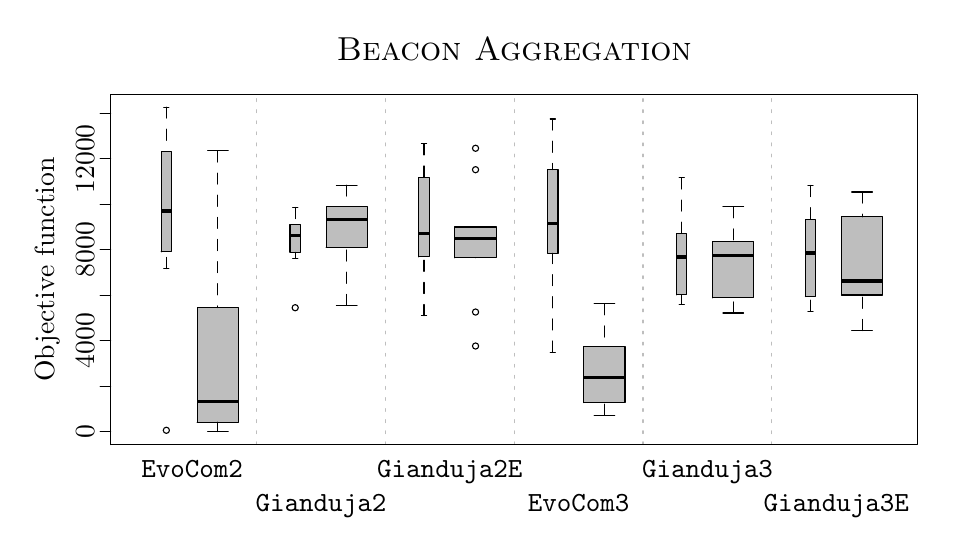
\begin{tikzpicture}[x=1pt,y=1pt]
\definecolor{fillColor}{RGB}{255,255,255}
\path[use as bounding box,fill=fillColor,fill opacity=0.00] (0,0) rectangle (325.21,180.67);
\begin{scope}
\path[clip] ( 30.00, 30.00) rectangle (321.61,156.67);
\definecolor{fillColor}{RGB}{190,190,190}

\path[fill=fillColor] ( 48.25, 99.63) --
	( 51.97, 99.63) --
	( 51.97,136.07) --
	( 48.25,136.07) --
	cycle;
\definecolor{drawColor}{RGB}{0,0,0}

\path[draw=drawColor,line width= 1.2pt,line join=round] ( 48.25,114.47) -- ( 51.97,114.47);

\path[draw=drawColor,line width= 0.4pt,dash pattern=on 4pt off 4pt ,line join=round,line cap=round] ( 50.11, 93.63) -- ( 50.11, 99.63);

\path[draw=drawColor,line width= 0.4pt,dash pattern=on 4pt off 4pt ,line join=round,line cap=round] ( 50.11,151.98) -- ( 50.11,136.07);

\path[draw=drawColor,line width= 0.4pt,line join=round,line cap=round] ( 49.18, 93.63) -- ( 51.04, 93.63);

\path[draw=drawColor,line width= 0.4pt,line join=round,line cap=round] ( 49.18,151.98) -- ( 51.04,151.98);

\path[draw=drawColor,line width= 0.4pt,line join=round,line cap=round] ( 48.25, 99.63) --
	( 51.97, 99.63) --
	( 51.97,136.07) --
	( 48.25,136.07) --
	( 48.25, 99.63);

\path[draw=drawColor,line width= 0.4pt,line join=round,line cap=round] ( 50.11, 35.18) circle (  1.12);

\path[fill=fillColor] ( 61.28, 38.12) --
	( 76.18, 38.12) --
	( 76.18, 79.55) --
	( 61.28, 79.55) --
	cycle;

\path[draw=drawColor,line width= 1.2pt,line join=round] ( 61.28, 45.60) -- ( 76.18, 45.60);

\path[draw=drawColor,line width= 0.4pt,dash pattern=on 4pt off 4pt ,line join=round,line cap=round] ( 68.73, 34.69) -- ( 68.73, 38.12);

\path[draw=drawColor,line width= 0.4pt,dash pattern=on 4pt off 4pt ,line join=round,line cap=round] ( 68.73,136.13) -- ( 68.73, 79.55);

\path[draw=drawColor,line width= 0.4pt,line join=round,line cap=round] ( 65.01, 34.69) -- ( 72.46, 34.69);

\path[draw=drawColor,line width= 0.4pt,line join=round,line cap=round] ( 65.01,136.13) -- ( 72.46,136.13);

\path[draw=drawColor,line width= 0.4pt,line join=round,line cap=round] ( 61.28, 38.12) --
	( 76.18, 38.12) --
	( 76.18, 79.55) --
	( 61.28, 79.55) --
	( 61.28, 38.12);

\path[fill=fillColor] ( 94.80, 99.50) --
	( 98.53, 99.50) --
	( 98.53,109.63) --
	( 94.80,109.63) --
	cycle;

\path[draw=drawColor,line width= 1.2pt,line join=round] ( 94.80,105.47) -- ( 98.53,105.47);

\path[draw=drawColor,line width= 0.4pt,dash pattern=on 4pt off 4pt ,line join=round,line cap=round] ( 96.67, 97.37) -- ( 96.67, 99.50);

\path[draw=drawColor,line width= 0.4pt,dash pattern=on 4pt off 4pt ,line join=round,line cap=round] ( 96.67,115.71) -- ( 96.67,109.63);

\path[draw=drawColor,line width= 0.4pt,line join=round,line cap=round] ( 95.73, 97.37) -- ( 97.60, 97.37);

\path[draw=drawColor,line width= 0.4pt,line join=round,line cap=round] ( 95.73,115.71) -- ( 97.60,115.71);

\path[draw=drawColor,line width= 0.4pt,line join=round,line cap=round] ( 94.80, 99.50) --
	( 98.53, 99.50) --
	( 98.53,109.63) --
	( 94.80,109.63) --
	( 94.80, 99.50);

\path[draw=drawColor,line width= 0.4pt,line join=round,line cap=round] ( 96.67, 79.48) circle (  1.12);

\path[fill=fillColor] (107.84,101.31) --
	(122.74,101.31) --
	(122.74,116.12) --
	(107.84,116.12) --
	cycle;

\path[draw=drawColor,line width= 1.2pt,line join=round] (107.84,111.26) -- (122.74,111.26);

\path[draw=drawColor,line width= 0.4pt,dash pattern=on 4pt off 4pt ,line join=round,line cap=round] (115.29, 80.32) -- (115.29,101.31);

\path[draw=drawColor,line width= 0.4pt,dash pattern=on 4pt off 4pt ,line join=round,line cap=round] (115.29,123.78) -- (115.29,116.12);

\path[draw=drawColor,line width= 0.4pt,line join=round,line cap=round] (111.56, 80.32) -- (119.01, 80.32);

\path[draw=drawColor,line width= 0.4pt,line join=round,line cap=round] (111.56,123.78) -- (119.01,123.78);

\path[draw=drawColor,line width= 0.4pt,line join=round,line cap=round] (107.84,101.31) --
	(122.74,101.31) --
	(122.74,116.12) --
	(107.84,116.12) --
	(107.84,101.31);

\path[fill=fillColor] (141.36, 97.84) --
	(145.08, 97.84) --
	(145.08,126.48) --
	(141.36,126.48) --
	cycle;

\path[draw=drawColor,line width= 1.2pt,line join=round] (141.36,106.38) -- (145.08,106.38);

\path[draw=drawColor,line width= 0.4pt,dash pattern=on 4pt off 4pt ,line join=round,line cap=round] (143.22, 76.62) -- (143.22, 97.84);

\path[draw=drawColor,line width= 0.4pt,dash pattern=on 4pt off 4pt ,line join=round,line cap=round] (143.22,138.70) -- (143.22,126.48);

\path[draw=drawColor,line width= 0.4pt,line join=round,line cap=round] (142.29, 76.62) -- (144.15, 76.62);

\path[draw=drawColor,line width= 0.4pt,line join=round,line cap=round] (142.29,138.70) -- (144.15,138.70);

\path[draw=drawColor,line width= 0.4pt,line join=round,line cap=round] (141.36, 97.84) --
	(145.08, 97.84) --
	(145.08,126.48) --
	(141.36,126.48) --
	(141.36, 97.84);

\path[fill=fillColor] (154.39, 97.54) --
	(169.29, 97.54) --
	(169.29,108.66) --
	(154.39,108.66) --
	cycle;

\path[draw=drawColor,line width= 1.2pt,line join=round] (154.39,104.60) -- (169.29,104.60);

\path[draw=drawColor,line width= 0.4pt,dash pattern=on 4pt off 4pt ,line join=round,line cap=round] (161.84, 97.54) -- (161.84, 97.54);

\path[draw=drawColor,line width= 0.4pt,dash pattern=on 4pt off 4pt ,line join=round,line cap=round] (161.84,108.66) -- (161.84,108.66);

\path[draw=drawColor,line width= 0.4pt,line join=round,line cap=round] (158.12, 97.54) -- (165.57, 97.54);

\path[draw=drawColor,line width= 0.4pt,line join=round,line cap=round] (158.12,108.66) -- (165.57,108.66);

\path[draw=drawColor,line width= 0.4pt,line join=round,line cap=round] (154.39, 97.54) --
	(169.29, 97.54) --
	(169.29,108.66) --
	(154.39,108.66) --
	(154.39, 97.54);

\path[draw=drawColor,line width= 0.4pt,line join=round,line cap=round] (161.84,137.09) circle (  1.12);

\path[draw=drawColor,line width= 0.4pt,line join=round,line cap=round] (161.84, 65.63) circle (  1.12);

\path[draw=drawColor,line width= 0.4pt,line join=round,line cap=round] (161.84,129.35) circle (  1.12);

\path[draw=drawColor,line width= 0.4pt,line join=round,line cap=round] (161.84, 77.91) circle (  1.12);

\path[fill=fillColor] (187.91, 99.14) --
	(191.64, 99.14) --
	(191.64,129.39) --
	(187.91,129.39) --
	cycle;

\path[draw=drawColor,line width= 1.2pt,line join=round] (187.91,109.79) -- (191.64,109.79);

\path[draw=drawColor,line width= 0.4pt,dash pattern=on 4pt off 4pt ,line join=round,line cap=round] (189.77, 63.44) -- (189.77, 99.14);

\path[draw=drawColor,line width= 0.4pt,dash pattern=on 4pt off 4pt ,line join=round,line cap=round] (189.77,147.65) -- (189.77,129.39);

\path[draw=drawColor,line width= 0.4pt,line join=round,line cap=round] (188.84, 63.44) -- (190.70, 63.44);

\path[draw=drawColor,line width= 0.4pt,line join=round,line cap=round] (188.84,147.65) -- (190.70,147.65);

\path[draw=drawColor,line width= 0.4pt,line join=round,line cap=round] (187.91, 99.14) --
	(191.64, 99.14) --
	(191.64,129.39) --
	(187.91,129.39) --
	(187.91, 99.14);

\path[fill=fillColor] (200.95, 45.23) --
	(215.84, 45.23) --
	(215.84, 65.57) --
	(200.95, 65.57) --
	cycle;

\path[draw=drawColor,line width= 1.2pt,line join=round] (200.95, 54.26) -- (215.84, 54.26);

\path[draw=drawColor,line width= 0.4pt,dash pattern=on 4pt off 4pt ,line join=round,line cap=round] (208.40, 40.59) -- (208.40, 45.23);

\path[draw=drawColor,line width= 0.4pt,dash pattern=on 4pt off 4pt ,line join=round,line cap=round] (208.40, 80.89) -- (208.40, 65.57);

\path[draw=drawColor,line width= 0.4pt,line join=round,line cap=round] (204.67, 40.59) -- (212.12, 40.59);

\path[draw=drawColor,line width= 0.4pt,line join=round,line cap=round] (204.67, 80.89) -- (212.12, 80.89);

\path[draw=drawColor,line width= 0.4pt,line join=round,line cap=round] (200.95, 45.23) --
	(215.84, 45.23) --
	(215.84, 65.57) --
	(200.95, 65.57) --
	(200.95, 45.23);

\path[fill=fillColor] (234.47, 84.09) --
	(238.19, 84.09) --
	(238.19,106.29) --
	(234.47,106.29) --
	cycle;

\path[draw=drawColor,line width= 1.2pt,line join=round] (234.47, 97.85) -- (238.19, 97.85);

\path[draw=drawColor,line width= 0.4pt,dash pattern=on 4pt off 4pt ,line join=round,line cap=round] (236.33, 80.67) -- (236.33, 84.09);

\path[draw=drawColor,line width= 0.4pt,dash pattern=on 4pt off 4pt ,line join=round,line cap=round] (236.33,126.38) -- (236.33,106.29);

\path[draw=drawColor,line width= 0.4pt,line join=round,line cap=round] (235.40, 80.67) -- (237.26, 80.67);

\path[draw=drawColor,line width= 0.4pt,line join=round,line cap=round] (235.40,126.38) -- (237.26,126.38);

\path[draw=drawColor,line width= 0.4pt,line join=round,line cap=round] (234.47, 84.09) --
	(238.19, 84.09) --
	(238.19,106.29) --
	(234.47,106.29) --
	(234.47, 84.09);

\path[fill=fillColor] (247.50, 83.01) --
	(262.40, 83.01) --
	(262.40,103.53) --
	(247.50,103.53) --
	cycle;

\path[draw=drawColor,line width= 1.2pt,line join=round] (247.50, 98.32) -- (262.40, 98.32);

\path[draw=drawColor,line width= 0.4pt,dash pattern=on 4pt off 4pt ,line join=round,line cap=round] (254.95, 77.56) -- (254.95, 83.01);

\path[draw=drawColor,line width= 0.4pt,dash pattern=on 4pt off 4pt ,line join=round,line cap=round] (254.95,115.98) -- (254.95,103.53);

\path[draw=drawColor,line width= 0.4pt,line join=round,line cap=round] (251.23, 77.56) -- (258.67, 77.56);

\path[draw=drawColor,line width= 0.4pt,line join=round,line cap=round] (251.23,115.98) -- (258.67,115.98);

\path[draw=drawColor,line width= 0.4pt,line join=round,line cap=round] (247.50, 83.01) --
	(262.40, 83.01) --
	(262.40,103.53) --
	(247.50,103.53) --
	(247.50, 83.01);

\path[fill=fillColor] (281.02, 83.50) --
	(284.74, 83.50) --
	(284.74,111.25) --
	(281.02,111.25) --
	cycle;

\path[draw=drawColor,line width= 1.2pt,line join=round] (281.02, 99.21) -- (284.74, 99.21);

\path[draw=drawColor,line width= 0.4pt,dash pattern=on 4pt off 4pt ,line join=round,line cap=round] (282.88, 78.24) -- (282.88, 83.50);

\path[draw=drawColor,line width= 0.4pt,dash pattern=on 4pt off 4pt ,line join=round,line cap=round] (282.88,123.63) -- (282.88,111.25);

\path[draw=drawColor,line width= 0.4pt,line join=round,line cap=round] (281.95, 78.24) -- (283.81, 78.24);

\path[draw=drawColor,line width= 0.4pt,line join=round,line cap=round] (281.95,123.63) -- (283.81,123.63);

\path[draw=drawColor,line width= 0.4pt,line join=round,line cap=round] (281.02, 83.50) --
	(284.74, 83.50) --
	(284.74,111.25) --
	(281.02,111.25) --
	(281.02, 83.50);

\path[fill=fillColor] (294.05, 84.08) --
	(308.95, 84.08) --
	(308.95,112.34) --
	(294.05,112.34) --
	cycle;

\path[draw=drawColor,line width= 1.2pt,line join=round] (294.05, 89.10) -- (308.95, 89.10);

\path[draw=drawColor,line width= 0.4pt,dash pattern=on 4pt off 4pt ,line join=round,line cap=round] (301.50, 71.25) -- (301.50, 84.08);

\path[draw=drawColor,line width= 0.4pt,dash pattern=on 4pt off 4pt ,line join=round,line cap=round] (301.50,121.30) -- (301.50,112.34);

\path[draw=drawColor,line width= 0.4pt,line join=round,line cap=round] (297.78, 71.25) -- (305.23, 71.25);

\path[draw=drawColor,line width= 0.4pt,line join=round,line cap=round] (297.78,121.30) -- (305.23,121.30);

\path[draw=drawColor,line width= 0.4pt,line join=round,line cap=round] (294.05, 84.08) --
	(308.95, 84.08) --
	(308.95,112.34) --
	(294.05,112.34) --
	(294.05, 84.08);
\definecolor{drawColor}{RGB}{190,190,190}

\path[draw=drawColor,line width= 0.4pt,dash pattern=on 1pt off 3pt ,line join=round,line cap=round] ( 82.70, 30.00) -- ( 82.70,156.67);

\path[draw=drawColor,line width= 0.4pt,dash pattern=on 1pt off 3pt ,line join=round,line cap=round] (129.25, 30.00) -- (129.25,156.67);

\path[draw=drawColor,line width= 0.4pt,dash pattern=on 1pt off 3pt ,line join=round,line cap=round] (175.81, 30.00) -- (175.81,156.67);

\path[draw=drawColor,line width= 0.4pt,dash pattern=on 1pt off 3pt ,line join=round,line cap=round] (222.36, 30.00) -- (222.36,156.67);

\path[draw=drawColor,line width= 0.4pt,dash pattern=on 1pt off 3pt ,line join=round,line cap=round] (268.92, 30.00) -- (268.92,156.67);
\end{scope}
\begin{scope}
\path[clip] (  0.00,  0.00) rectangle (325.21,180.67);
\definecolor{drawColor}{RGB}{0,0,0}

\node[text=drawColor,anchor=base,inner sep=0pt, outer sep=0pt, scale=  1.00] at ( 59.42, 18.00) {\texttt{EvoCom2}};

\node[text=drawColor,anchor=base,inner sep=0pt, outer sep=0pt, scale=  1.00] at (152.53, 18.00) {\texttt{Gianduja2E}};

\node[text=drawColor,anchor=base,inner sep=0pt, outer sep=0pt, scale=  1.00] at (245.64, 18.00) {\texttt{Gianduja3}};

\node[text=drawColor,anchor=base,inner sep=0pt, outer sep=0pt, scale=  1.00] at (105.98,  6.00) {\texttt{Gianduja2}};

\node[text=drawColor,anchor=base,inner sep=0pt, outer sep=0pt, scale=  1.00] at (199.08,  6.00) {\texttt{EvoCom3}};

\node[text=drawColor,anchor=base,inner sep=0pt, outer sep=0pt, scale=  1.00] at (292.19,  6.00) {\texttt{Gianduja3E}};
\end{scope}
\begin{scope}
\path[clip] (  0.00,  0.00) rectangle (325.21,180.67);
\definecolor{drawColor}{RGB}{0,0,0}

\node[text=drawColor,anchor=base,inner sep=0pt, outer sep=0pt, scale=  1.20] at (175.81,168.67) {\textsc{Beacon Aggregation}};

\node[text=drawColor,rotate= 90.00,anchor=base,inner sep=0pt, outer sep=0pt, scale=  1.00] at (  9.60, 93.34) {Objective function};
\end{scope}
\begin{scope}
\path[clip] (  0.00,  0.00) rectangle (325.21,180.67);
\definecolor{drawColor}{RGB}{0,0,0}

\path[draw=drawColor,line width= 0.4pt,line join=round,line cap=round] ( 30.00, 34.68) -- ( 30.00,149.72);

\path[draw=drawColor,line width= 0.4pt,line join=round,line cap=round] ( 30.00, 34.68) -- ( 26.20, 34.68);

\path[draw=drawColor,line width= 0.4pt,line join=round,line cap=round] ( 30.00, 51.12) -- ( 26.20, 51.12);

\path[draw=drawColor,line width= 0.4pt,line join=round,line cap=round] ( 30.00, 67.55) -- ( 26.20, 67.55);

\path[draw=drawColor,line width= 0.4pt,line join=round,line cap=round] ( 30.00, 83.99) -- ( 26.20, 83.99);

\path[draw=drawColor,line width= 0.4pt,line join=round,line cap=round] ( 30.00,100.42) -- ( 26.20,100.42);

\path[draw=drawColor,line width= 0.4pt,line join=round,line cap=round] ( 30.00,116.85) -- ( 26.20,116.85);

\path[draw=drawColor,line width= 0.4pt,line join=round,line cap=round] ( 30.00,133.29) -- ( 26.20,133.29);

\path[draw=drawColor,line width= 0.4pt,line join=round,line cap=round] ( 30.00,149.72) -- ( 26.20,149.72);

\node[text=drawColor,rotate= 90.00,anchor=base,inner sep=0pt, outer sep=0pt, scale=  1.00] at ( 24.00, 34.68) {0};

\node[text=drawColor,rotate= 90.00,anchor=base,inner sep=0pt, outer sep=0pt, scale=  1.00] at ( 24.00, 67.55) {4000};

\node[text=drawColor,rotate= 90.00,anchor=base,inner sep=0pt, outer sep=0pt, scale=  1.00] at ( 24.00,100.42) {8000};

\node[text=drawColor,rotate= 90.00,anchor=base,inner sep=0pt, outer sep=0pt, scale=  1.00] at ( 24.00,133.29) {12000};

\path[draw=drawColor,line width= 0.4pt,line join=round,line cap=round] ( 30.00, 30.00) --
	(321.61, 30.00) --
	(321.61,156.67) --
	( 30.00,156.67) --
	( 30.00, 30.00);
\end{scope}
\end{tikzpicture}
